% ============================================================
%  CAPÍTULO 6 — RESULTADOS EXPERIMENTALES
%  Memoria TFG: Transcripción automática de música de piano
%  Autor: María Piedad Castex Sierra
% ============================================================

\chapter{Resultados Experimentales}
\label{cap:resultados}

El presente capítulo describe el protocolo de evaluación aplicado,
presenta las curvas de entrenamiento obtenidas durante los experimentos
y reporta las métricas cuantitativas sobre el conjunto de prueba del
corpus MAESTRO. Se analiza a continuación el comportamiento diferencial
de los tres modelos entrenados y se contextualiza su rendimiento en
relación con el estado del arte.

% -----------------------------------------------------------
\section{Protocolo de evaluación}
\label{sec:protocolo_evaluacion}
% -----------------------------------------------------------

La evaluación cuantitativa se realizó sobre una muestra aleatoria de
30 piezas del conjunto de prueba oficial de MAESTRO
(semilla fija $s = 42$), extraída del total de 125 interpretaciones
del \textit{split} de prueba (véase Tabla~\ref{tab:maestro_splits}).
El tamaño muestral se limitó a 30 piezas por las restricciones de
tiempo de cómputo del entorno Google Colaboratory; la selección
aleatoria con semilla fija garantiza la reproducibilidad del resultado.

% CORREGIDO: el criterio real de selección fue el ranking por
% val_loss que Colab añade al nombre de archivo, no F1.
Para \texttt{v1\_baseline} y \texttt{exp02\_short\_clips}, el
\textit{checkpoint} evaluado se determinó de forma manual a partir
del sufijo de ranking por pérdida de validación que Google
Colaboratory añade automáticamente al nombre de los archivos de
\textit{checkpoint} guardados (p.\,ej.\ \texttt{-001}, \texttt{-002},
\ldots); en cada caso se seleccionó el \textit{checkpoint} mejor
posicionado en dicho ranking. Para \texttt{exp01\_reduced\_data} este
mecanismo de ranking no estuvo disponible, por lo que se empleó
directamente el \textit{checkpoint} de la última época del
entrenamiento (época~514). En ningún caso se conservó un registro
numérico exportable de la pérdida de validación por época, por lo que
las curvas presentadas en la Sección~\ref{sec:curvas_entrenamiento}
no incluyen dicha señal; el criterio empleado para seleccionar el
\textit{checkpoint} y las métricas F1 analizadas en esa sección
proceden, por tanto, de dos fuentes de información distintas.

La estrategia de decodificación empleada en todos los casos fue el
muestreo con temperatura $\tau = 0.8$, tal y como se describió en la
Sección~\ref{sec:inferencia_evaluacion}.

Las métricas calculadas con \texttt{mir\_eval} son las tres variantes
a nivel de nota definidas en la Sección~\ref{sec:metricas}: F1 de
\textit{onset} (tolerancia $\pm 50\,\mathrm{ms}$), F1 de
\textit{onset} + \textit{offset} ($\pm 50\,\mathrm{ms}$ o 0.2 de
la duración) y F1 de \textit{onset} + velocidad ($\pm 50\,\mathrm{ms}$
más tolerancia del 0.1 en velocidad).

% -----------------------------------------------------------
\section{Curvas de entrenamiento}
\label{sec:curvas_entrenamiento}
% -----------------------------------------------------------

% CORREGIDO: aclara que la selección no se basó en las métricas F1
% que se presentan a continuación.
Para cada configuración experimental se registró la evolución de la
pérdida de entrenamiento y de las métricas F1 sobre el conjunto de
validación. Como se ha indicado en la
Sección~\ref{sec:protocolo_evaluacion}, el \textit{checkpoint}
evaluado en \texttt{v1\_baseline} y \texttt{exp02\_short\_clips} se
seleccionó de forma manual a partir del ranking por pérdida de
validación generado automáticamente por Google Colaboratory, y no a
partir de las métricas F1 que se presentan a continuación; en
\texttt{exp01\_reduced\_data}, al no disponer de dicho ranking, se
empleó el \textit{checkpoint} de la última época. Esta distinción es
relevante para interpretar correctamente las figuras siguientes: el
punto marcado como mejor \textit{checkpoint} no tiene por qué
coincidir con el máximo de F1 visible en cada gráfica, puesto que
ambas señales --pérdida de validación y F1-- se calcularon de forma
independiente y no necesariamente evolucionan de forma idéntica.

\subsection{v1\_baseline}
\label{subsec:v1_baseline}

\begin{figure}[htbp]
    \centering
    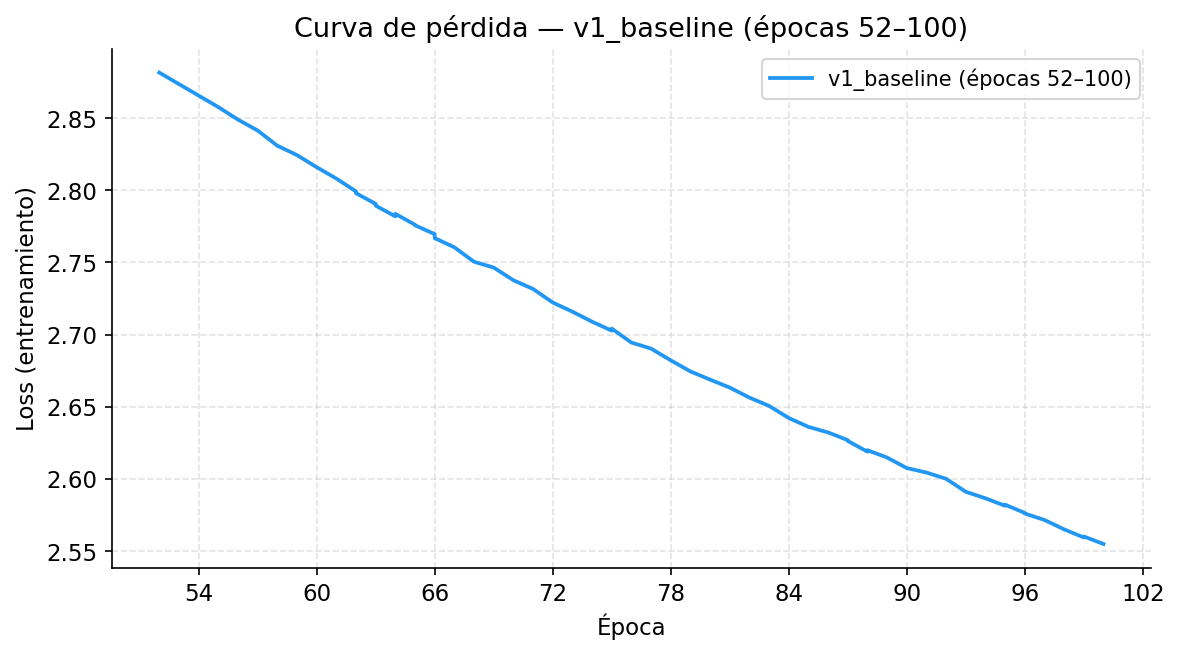
\includegraphics[width=0.92\textwidth]{figs/loss_v1_baseline.png}
    \caption{Evolución de la pérdida de entrenamiento de
    \texttt{v1\_baseline} entre las épocas 52 y 100 (corpus
    completo, \texttt{MAX\_AUDIO\_FRAMES} = 4\,096).}
    \label{fig:curva_baseline}
\end{figure}

La pérdida de entrenamiento (Figura~\ref{fig:curva_baseline}) presenta
las siguientes características en el tramo disponible:

\begin{itemize}
    \item \textbf{Rango:} desciende de 2.88 (época~52) a
    aproximadamente 2.56 (época~98--100).
    \item \textbf{Forma:} descenso prácticamente monótono, sin ruido
    apreciable.
    \item \textbf{Cobertura:} no hay registro de las primeras 52
    épocas, por lo que no puede describirse el comportamiento inicial
    del entrenamiento.
\end{itemize}


\begin{figure}[htbp]
    \centering
    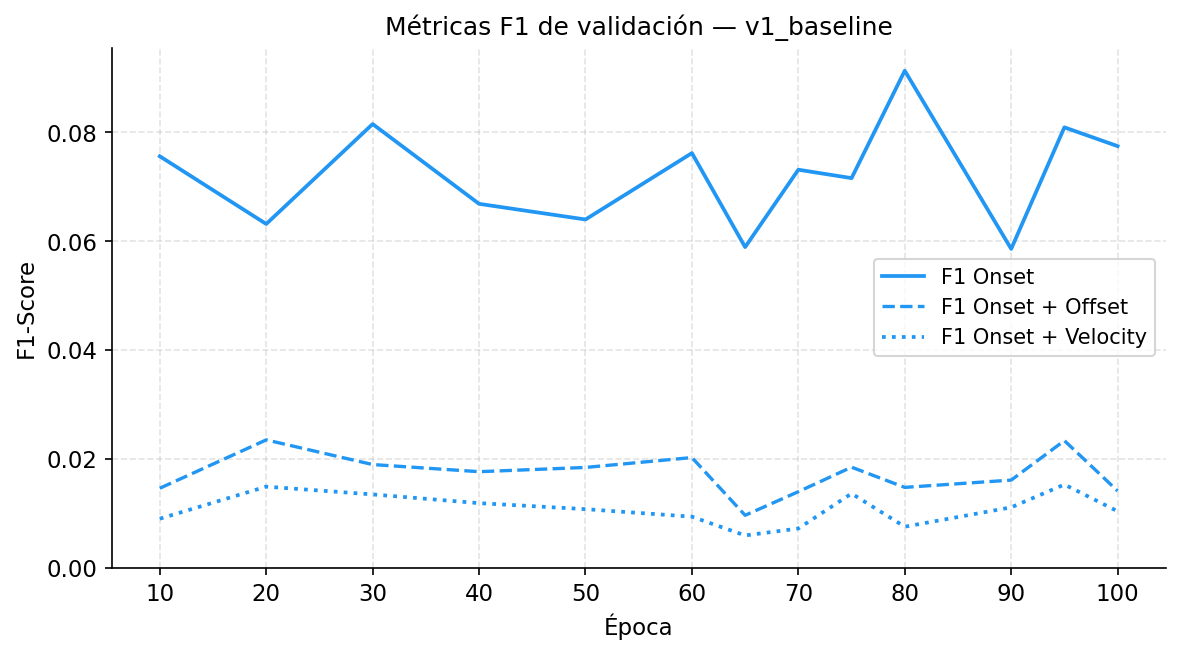
\includegraphics[width=0.92\textwidth]{figs/f1_v1_baseline.png}
    \caption{Métricas F1 de validación de \texttt{v1\_baseline}.
    El mejor \textit{checkpoint} corresponde a la época~98.}
    \label{fig:f1_baseline}
\end{figure}

La evolución del F1 de validación (Figura~\ref{fig:f1_baseline})
contrasta con la suavidad de la curva de pérdida:

\begin{itemize}
    \item \textbf{F1 \textit{onset}:} oscila entre 0.059 y 0.091 sin
    tendencia de mejora sostenida; máximo en la época~80, mínimos
    locales en las épocas~65 y~90.
    \item \textbf{F1 \textit{onset+offset}:} se mantiene en una banda
    estrecha de 0.010--0.023 durante todo el entrenamiento.
    \item \textbf{F1 \textit{onset+velocity}:} banda de 0.006--0.015.
    \item \textbf{\textit{Checkpoint} evaluado (época~98):}
    seleccionado por su posición en el ranking de pérdida de
    validación de Colaboratory, no por F1. Los valores vecinos
    (épocas~95 y~100) son 0.081 y 0.077 respectivamente. Esto representa una franja
    de F1 alta pero no máxima, ya que el pico de la curva (0.091) se
    da en la época~80.
\end{itemize}

Esta discrepancia entre una pérdida de entrenamiento que mejora de
forma constante y un F1 de validación mucho más ruidoso sugiere que,
en este experimento, la reducción continuada de la pérdida no se
traduce necesariamente en una mejora proporcional y estable de la
calidad de la transcripción. La cercanía entre el \textit{checkpoint}
elegido por pérdida de validación y una zona de F1 razonablemente alta
es, sin ser una coincidencia exacta, una señal tranquilizadora de que
ambos criterios no divergen de forma severa en este experimento.

\clearpage

\subsection{exp01\_reduced\_data}
\label{subsec:exp01}

\begin{figure}[htbp]
    \centering
    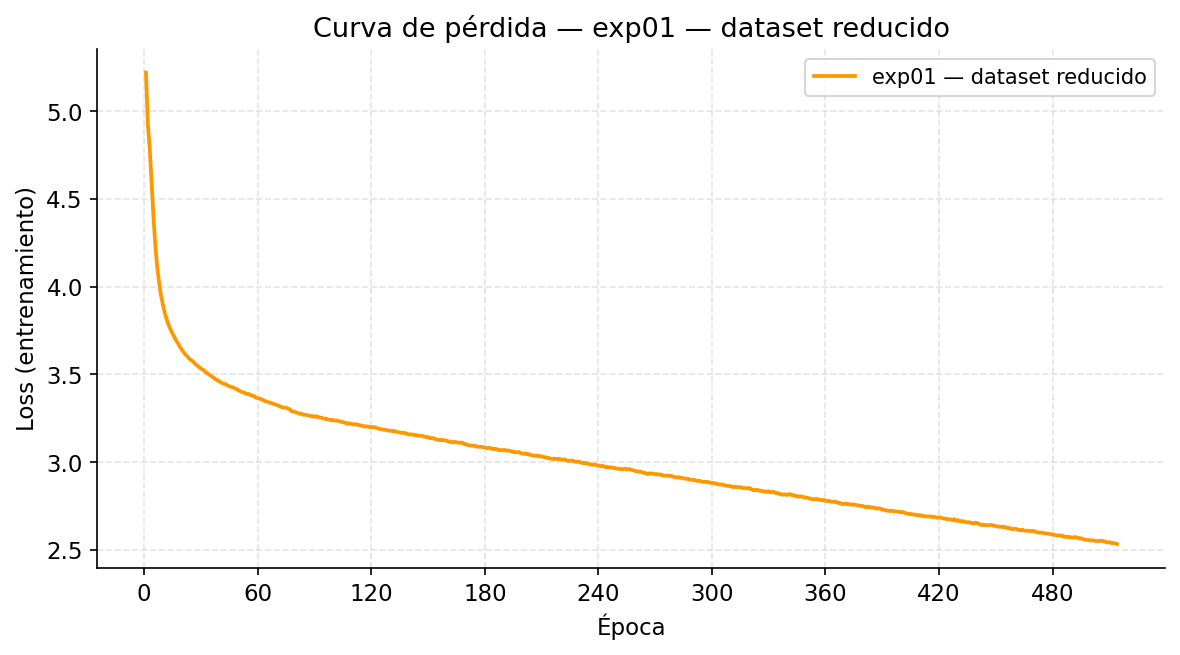
\includegraphics[width=0.92\textwidth]{figs/loss_exp01_reduced_data.png}
    \caption{Evolución de la pérdida de entrenamiento de
    \texttt{exp01\_reduced\_data} (150 muestras de entrenamiento).}
    \label{fig:curva_exp01}
\end{figure}

El modelo correspondiente a \texttt{exp01\_reduced\_data} entrenó con solo 150 muestras. Su curva
de pérdida de entrenamiento (Figura~\ref{fig:curva_exp01}) muestra:

\begin{itemize}
    \item \textbf{Rango:} de 5.25 (época~0) a 2.53 (época~514).
    \item \textbf{Caída inicial:} descenso rápido hasta $\approx$3.5
    en las primeras 30--40 épocas.
    \item \textbf{Tramo final:} descenso lento y prácticamente lineal
    durante el resto del entrenamiento, sin señales de estancamiento.
\end{itemize}

Este descenso sostenido durante más de 500 épocas, típico de un
escenario de sobreajuste a un conjunto de datos reducido, no puede
contrastarse directamente con una curva de pérdida de validación, al
no haberse conservado un registro numérico de esta última.
\clearpage
\begin{figure}[htbp]
    \centering
    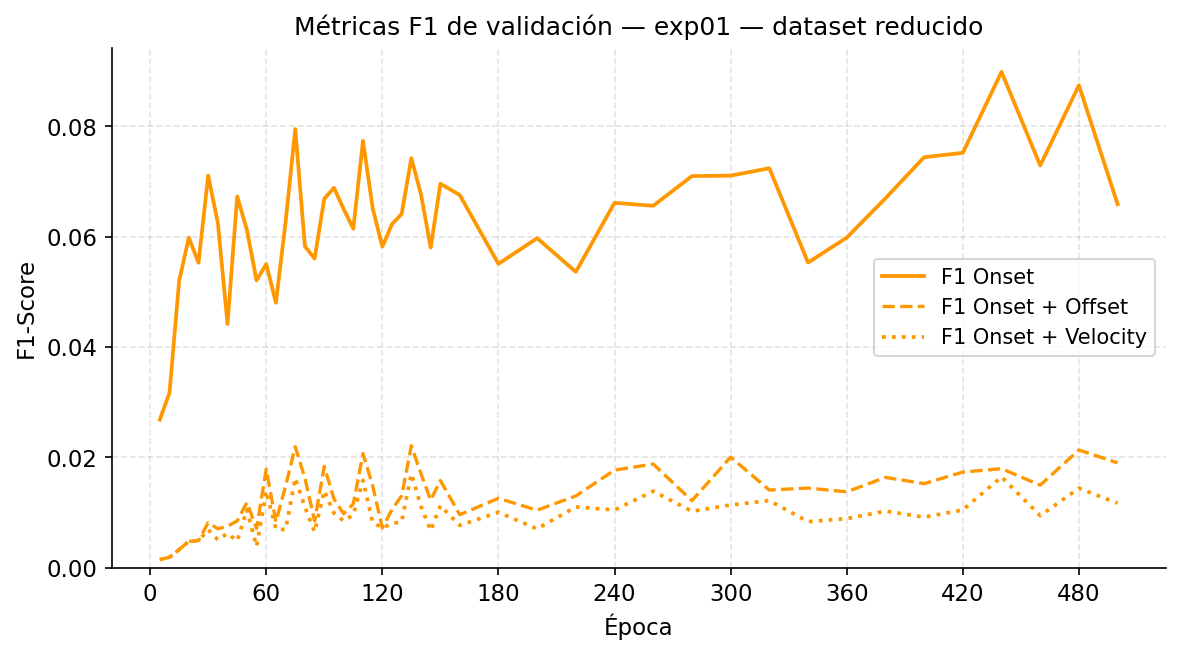
\includegraphics[width=0.92\textwidth]{figs/f1_exp01_reduced_data.png}
    \caption{Métricas F1 de validación de
    \texttt{exp01\_reduced\_data}. Se empleó el
    \textit{checkpoint} de la última época disponible (514) al no
    disponer de ranking de pérdida de validación.}
    \label{fig:f1_exp01}
\end{figure}

Las métricas F1 de validación (Figura~\ref{fig:f1_exp01}) matizan
esta lectura:

\begin{itemize}
    \item \textbf{Subida inicial:} rápida durante las primeras
    30--40 épocas.
    \item \textbf{F1 \textit{onset}:} oscila con varianza
    considerable en una banda de 0.05--0.09, con ligera tendencia
    ascendente hacia el final; máximos globales en torno a las
    épocas~430 y~480 ($\approx$0.090 y $\approx$0.087).
    \item \textbf{F1 \textit{onset+offset} y \textit{onset+velocity}:}
    patrón similar, con magnitudes menores.
    \item \textbf{\textit{Checkpoint} evaluado (época~514):} sin
    ranking de pérdida de validación disponible, se empleó
    directamente la última época --el único de los tres experimentos
    sin ningún criterio de rendimiento asociado. Su F1
    \textit{onset} ($\approx$0.066) cae en un valle local,
    sensiblemente por debajo de los picos observados 30--80 épocas
    antes.
\end{itemize}

Esta tendencia no muestra la degradación de F1 que cabría esperar de
un sobreajuste severo. El desajuste entre el punto de máximo
rendimiento observado durante el entrenamiento y el \textit{checkpoint}
efectivamente utilizado constituye una explicación plausible,
adicional a la limitada capacidad de generalización propia de un
conjunto de entrenamiento tan reducido, de por qué
\texttt{exp01\_reduced\_data} obtiene los resultados más bajos de los
tres experimentos sobre el conjunto de \textit{test} (F1
\textit{onset} de 0.065, con solo 1 de 30 piezas alcanzando un F1
superior a 0.10).

\clearpage

\subsection{exp02\_short\_clips}
\label{subsec:exp02}

\begin{figure}[htbp]
    \centering
    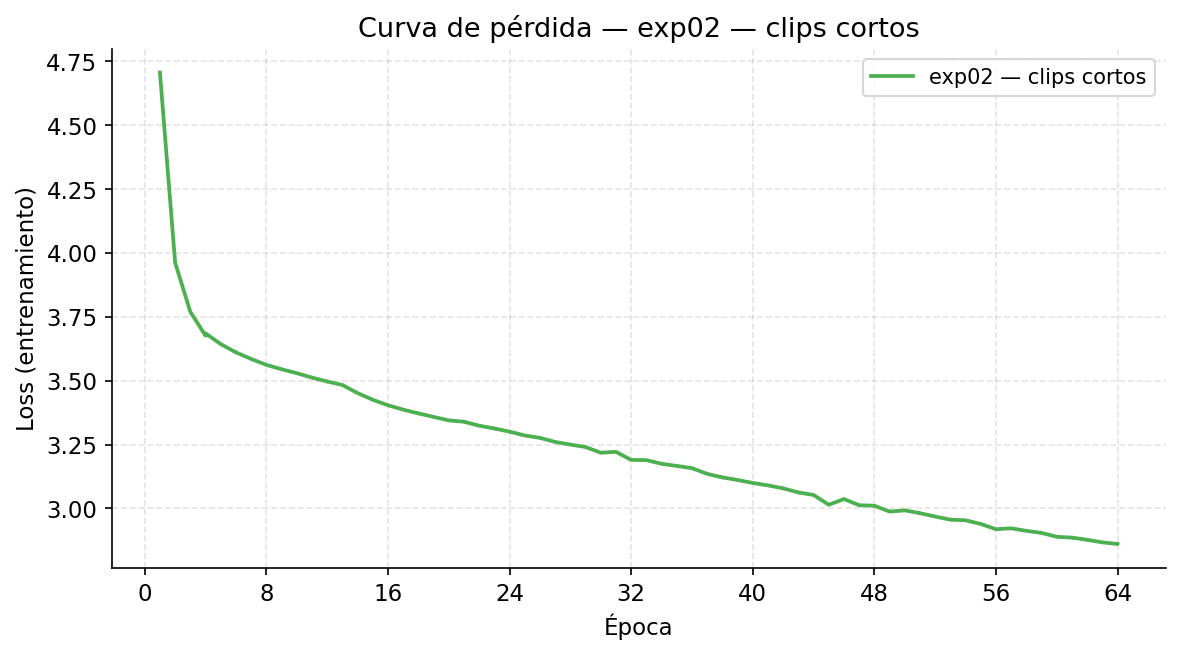
\includegraphics[width=0.92\textwidth]{figs/loss_exp02_short_clips.png}
    \caption{Evolución de la pérdida de entrenamiento de
    \texttt{exp02\_short\_clips} (corpus completo,
    \texttt{MAX\_AUDIO\_FRAMES} = 2\,048).}
    \label{fig:curva_exp02}
\end{figure}

La curva de pérdida de entrenamiento (Figura~\ref{fig:curva_exp02})
presenta:

\begin{itemize}
    \item \textbf{Rango:} de 4.7 (época~0) a 2.85 (época~64).
    \item \textbf{Caída inicial:} pronunciada, hasta $\approx$3.7 en
    las primeras 5 épocas.
    \item \textbf{Tramo posterior:} descenso continuo y suave, sin
    estancamiento ni repuntes en el registro disponible.
\end{itemize}

\begin{figure}[htbp]
    \centering
    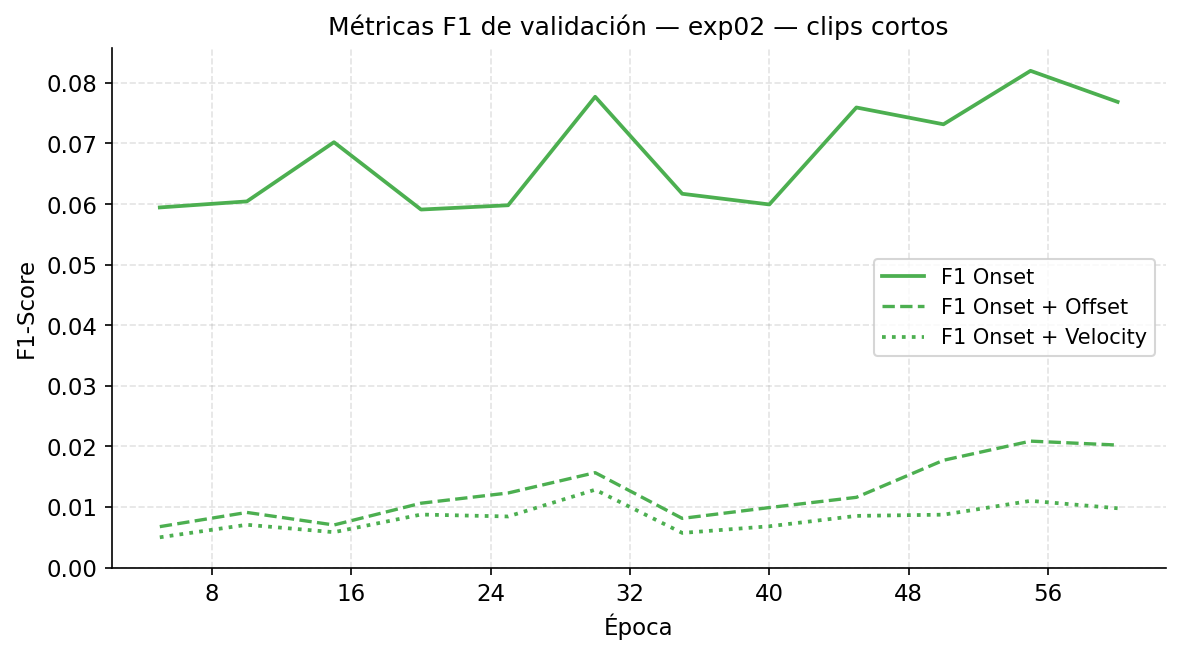
\includegraphics[width=0.92\textwidth]{figs/f1_exp02_short_clips.png}
    \caption{Métricas F1 de validación de
    \texttt{exp02\_short\_clips}. El mejor \textit{checkpoint}
    corresponde a la época~57.}
    \label{fig:f1_exp02}
\end{figure}

El F1 de validación (Figura~\ref{fig:f1_exp02}) también mejora de
forma sostenida, aunque ruidosa:

\begin{itemize}
    \item \textbf{F1 \textit{onset}:} sube de $\approx$0.06 (épocas
    iniciales) a un máximo de $\approx$0.082 hacia la época~56.
    \item \textbf{F1 \textit{onset+offset}:} tendencia ascendente
    clara en la segunda mitad del entrenamiento, de $\approx$0.008
    (época~35) a $\approx$0.021 (época~55).
    \item \textbf{\textit{Checkpoint} evaluado (época~57):}
    seleccionado por el ranking de pérdida de validación de
    Colaboratory, no directamente por F1; cae muy cerca de los
    valores más altos de F1 observados en el rango registrado.
\end{itemize}

Ni la pérdida de entrenamiento ni el F1 de validación muestran
estancamiento o divergencia en torno a la época~57, ambas señales
evolucionan de forma consistente hasta donde alcanza el registro
disponible indicando que el entrenamiento se interrumpió  
mientras el modelo aún tenía capacidad de mejora, y no como consecuencia de una
degradación por sobreajuste detectable en estas curvas.

\subsection{Comparativa entre experimentos}
\label{subsec:comparativa}

\begin{figure}[htbp]
    \centering
    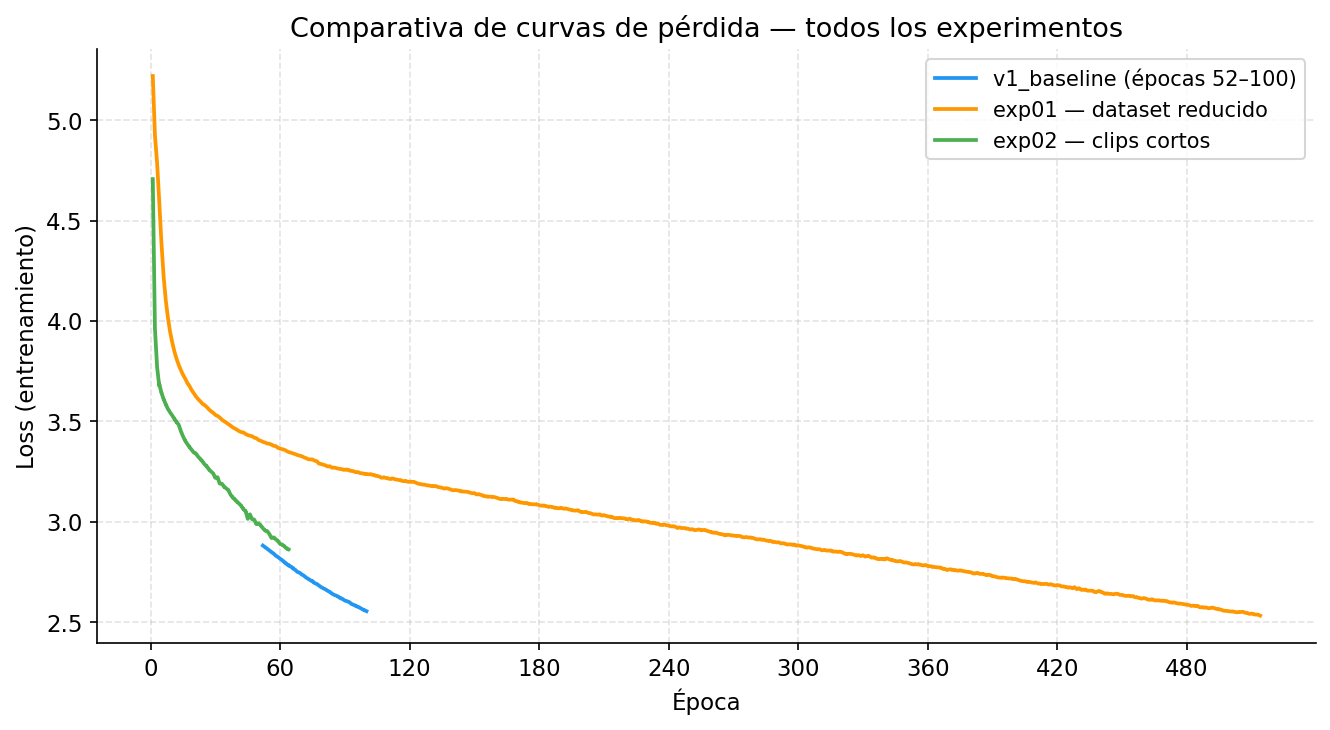
\includegraphics[width=0.92\textwidth]{figs/loss_all_experiments.png}
    \caption{Comparativa de las curvas de pérdida de
    entrenamiento de los tres experimentos.}
    \label{fig:comparativa_loss}
\end{figure}

\begin{figure}[htbp]
    \centering
    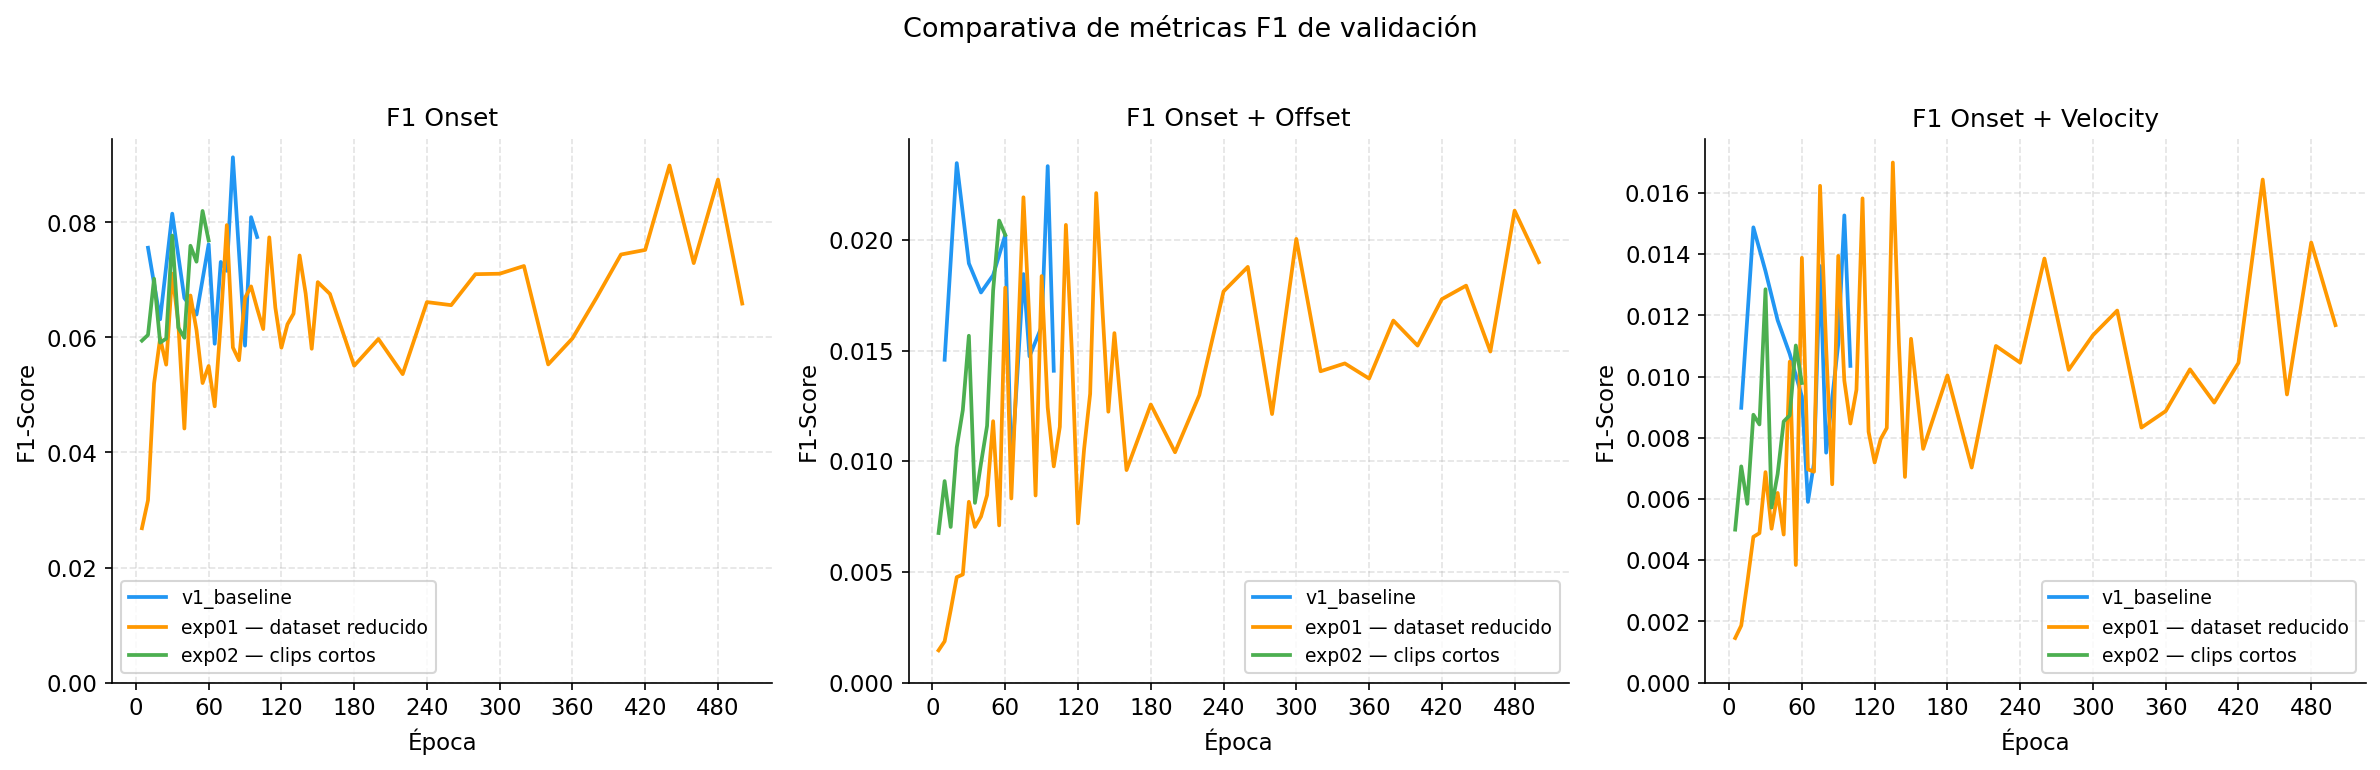
\includegraphics[width=0.95\textwidth]{figs/f1_all_experiments.png}
    \caption{Comparativa de las métricas F1 de validación
    (\textit{onset}, \textit{onset+offset} y
    \textit{onset+velocity}) de los tres experimentos.}
    \label{fig:comparativa_f1}
\end{figure}

Las Figuras~\ref{fig:comparativa_loss} y~\ref{fig:comparativa_f1}
permiten resumir las diferencias entre experimentos (ver siguiente página):

\begin{itemize}
    \item \textbf{Escala temporal:} \texttt{v1\_baseline} y
    \texttt{exp02\_short\_clips} completan su entrenamiento en un
    centenar de épocas; \texttt{exp01\_reduced\_data}, con muchas
    menos muestras por época, se extiende durante más de 500.
    \item \textbf{F1 \textit{onset} de validación:} rango comparable
    entre los tres experimentos ($\approx$0.06--0.09) durante sus
    respectivas fases de entrenamiento.
    \item \textbf{F1 \textit{onset+offset} y \textit{onset+velocity}:}
    muy por debajo del F1 \textit{onset} en los tres casos, en línea
    con la caída observada en \textit{test} entre \textit{onset} y
    las métricas combinadas: 0.665 (\texttt{v1\_baseline}),
    0.809 (\texttt{exp01\_reduced\_data}) y 0.750
    (\texttt{exp02\_short\_clips}).
    \item \textbf{Criterio de selección de \textit{checkpoint}:}
    \begin{itemize}
        \item \texttt{v1\_baseline} y \texttt{exp02\_short\_clips}:
        ranking automático por pérdida de validación de
        Colaboratory, razonablemente coherente con las métricas F1
        mostradas.
        \item \texttt{exp01\_reduced\_data}: ranking no disponible;
        se empleó la última época, sin ningún criterio de rendimiento
        asociado.
    \end{itemize}
\end{itemize}

Esta ausencia total de un criterio de selección en
\texttt{exp01\_reduced\_data} (y no solo la escasez de datos de
entrenamiento) constituye una explicación adicional y bien
fundamentada de su resultado comparativamente más bajo sobre el
conjunto de \textit{test}.

% -----------------------------------------------------------
\section{Análisis cualitativo}
\label{sec:analisis_cualitativo}
% -----------------------------------------------------------

La Tabla~\ref{tab:resultados_test} resume las métricas obtenidas por
cada modelo sobre las 30 piezas del conjunto de prueba, calculadas a
partir de los resultados individuales por pieza con \texttt{mir\_eval}.

\begin{table}[htbp]
    \centering
    \caption{Métricas de evaluación sobre el conjunto de prueba
    (30 piezas, semilla 42). Los valores se calculan pieza a pieza y
    se agregan mediante media y desviación típica.}
    \label{tab:resultados_test}
    \begin{tabular}{lccc}
        \toprule
        \textbf{Métrica} & \texttt{v1\_baseline} & \texttt{exp01} & \texttt{exp02} \\
        \midrule
        F1 \textit{onset} (media $\pm$ std) & $0.080 \pm 0.025$ & $0.065 \pm 0.018$ & $0.103 \pm 0.042$ \\
        F1 \textit{onset} (mediana) & 0.071 & 0.064 & 0.097 \\
        F1 \textit{onset} (rango) & 0.041--0.139 & 0.032--0.115 & 0.028--0.188 \\
        F1 \textit{onset+offset} (media $\pm$ std) & $0.029 \pm 0.017$ & $0.013 \pm 0.007$ & $0.029 \pm 0.022$ \\
        F1 \textit{onset+velocity} (media $\pm$ std) & $0.016 \pm 0.011$ & $0.007 \pm 0.005$ & $0.017 \pm 0.014$ \\
        Notas GT (media) & 877 & 877 & 450 \\
        Notas predichas (media) & 618 & 624 & 543 \\
        Ratio pred/GT (media por pieza) & 0.79 & 0.80 & 1.32 \\
        Piezas con F1 \textit{onset} $>$ 0.10 & 8/30 & 1/30 & 14/30 \\
        Piezas con F1 \textit{onset} $>$ 0.5 & 0/30 & 0/30 & 0/30 \\
        \bottomrule
    \end{tabular}
\end{table}

\subsection{Patrón de predicción de notas}

Los tres modelos exhiben comportamientos distintos en cuanto al
número de notas predichas respecto a la referencia:

\begin{itemize}
    \item \textbf{\texttt{v1\_baseline}:} infrapredice de forma
    consistente, generando en promedio el 0.79 de las notas de
    referencia (618 de 877 notas).
    \item \textbf{\texttt{exp01\_reduced\_data}:} presenta un patrón
    muy similar a \texttt{v1\_baseline}, con un 0.80 de las notas de
    referencia (624 de 877).
    \item \textbf{\texttt{exp02\_short\_clips}:} suprapredice, con un
    1.32 de las notas de referencia (543 de 450).
\end{itemize}

Antes de interpretar esta diferencia, es necesario señalar una
precaución metodológica: el promedio de notas GT de
\texttt{exp02\_short\_clips} (450) es aproximadamente la mitad del de
\texttt{v1\_baseline} y \texttt{exp01\_reduced\_data} (877 en ambos
casos), a pesar de evaluarse sobre las mismas 30 piezas. Esto no se
debe a que las piezas sean distintas, sino a que
\texttt{exp02\_short\_clips} trunca el audio a
\texttt{MAX\_AUDIO\_FRAMES} = 2\,048 (aproximadamente 41 segundos)
frente a los 4\,096 (aproximadamente 82 segundos) de los otros dos
modelos: la referencia MIDI utilizada en la evaluación se recorta a
la misma ventana temporal que ve el modelo, por lo que
\texttt{exp02\_short\_clips} se evalúa, en promedio, sobre menos de la
mitad de notas por pieza que los demás. En consecuencia, los recuentos
absolutos de notas de \texttt{exp02\_short\_clips} no son directamente
comparables con los de los otros dos experimentos; el ratio
predicción/referencia calculado \emph{dentro} de la ventana propia de
cada modelo sí lo es, y es el que sostiene la lectura anterior: los
modelos entrenados sobre clips largos tienden a la cautela, mientras
que el entrenado sobre clips cortos tiende a sobregenerar notas,
posiblemente porque los fragmentos breves de MAESTRO contienen una
proporción más alta de pasajes musicalmente activos que las piezas
completas, y el modelo aprendió a activar notas con mayor frecuencia
en consecuencia.

\subsection{Brecha entre onset y onset+offset}

Los tres modelos exhiben una caída sistemática del F1 al añadir la
exigencia de detección de \textit{offset}, calculada como la caída
porcentual media pieza a pieza:

\begin{itemize}
    \item \textbf{\texttt{v1\_baseline}:} caída del 0.665
    (F1 \textit{onset} de 0.080 a F1 \textit{onset+offset} de 0.029).
    \item \textbf{\texttt{exp02\_short\_clips}:} caída del 0.750
    (de 0.103 a 0.029).
    \item \textbf{\texttt{exp01\_reduced\_data}:} caída del 0.809
    la más pronunciada de los tres (de 0.065 a 0.013).
\end{itemize}

Este patrón indica que el sistema ha aprendido a detectar el inicio de
las notas con cierta consistencia, pero prácticamente no modela su
duración. Es coherente con las propiedades acústicas del problema: el
\textit{onset} produce un transitorio espectral distintivo y bien
localizado en el tiempo, mientras que el \textit{offset} depende del
decaimiento acústico y del pedal de resonancia; fenómenos de mayor
complejidad temporal que requieren capturar dependencias a largo
plazo, precisamente donde las restricciones de truncación y tamaño de
modelo limitan más al sistema. Que la caída sea máxima en
\texttt{exp01\_reduced\_data}, el experimento con menos datos de
entrenamiento, es consistente con esta lectura: modelar el
\textit{offset} exige generalizar patrones de duración de nota más
sutiles que el propio \textit{onset}, y es razonable que sea la
capacidad más perjudicada por la escasez de datos.

\subsection{Efecto de la longitud del clip de entrenamiento}

\texttt{exp02\_short\_clips} obtiene el mejor F1 de \textit{onset}
medio (0.103) y el mayor número de piezas por encima del umbral de
0.10 (14 de 30), pese a entrenarse con secuencias de la mitad de
duración que \texttt{v1\_baseline}. Dos factores, no excluyentes,
pueden explicar esta mejora:

\begin{itemize}
    \item \textbf{Densidad de señal de aprendizaje:} los clips de
    41 segundos contienen, en proporción, menos silencio inicial y
    más eventos musicales activos que las piezas completas de
    MAESTRO, lo que mejora la densidad de señal de aprendizaje por
    época.
    \item \textbf{Mayor número de épocas efectivas:} al procesar
    secuencias más cortas, \newline\texttt{exp02\_short\_clips} completó más
    pasos de optimización por época que \texttt{v1\_baseline} en un
    tiempo de cómputo comparable.
\end{itemize}

Este beneficio tiene, no obstante, un coste: la incapacidad del
modelo para aprender dependencias estructurales a mayor escala
temporal, lo que --como se discute en el apartado anterior-- puede
explicar tanto su mayor caída relativa de F1 al añadir el
\textit{offset} respecto a \texttt{v1\_baseline}, como su tendencia a
suprapredecir notas al generalizar a piezas completas durante la
evaluación, un contexto de duración muy distinto al de entrenamiento.

\subsection{Varianza entre piezas}

Los tres modelos presentan una desviación típica considerable en el
F1 de \textit{onset}, especialmente \texttt{exp02\_short\_clips}
($\sigma = 0.042$, frente a $\sigma = 0.025$ en
\texttt{v1\_baseline} y $\sigma = 0.018$ en
\texttt{exp01\_reduced\_data}), con un rango de valores que va de
0.028 a 0.188 según la pieza. El cruce de los resultados por pieza
entre modelos aporta dos observaciones concretas sobre el origen de
esta variabilidad:

\begin{itemize}
    \item \textbf{Dificultad compartida entre configuraciones:} el F1
    de \textit{onset} por pieza está correlacionado entre modelos;
    fuertemente entre \texttt{v1\_baseline} y
    \texttt{exp02\_short\_clips} ($r = 0.71$), moderadamente entre
    \texttt{v1\_baseline} y \texttt{exp01\_reduced\_data}
    ($r = 0.38$); lo que indica que una parte de la variabilidad
    responde a características intrínsecas de cada pieza, no solo a
    la configuración del modelo. De hecho, la pieza peor transcrita
    por \texttt{v1\_baseline} (F1 = 0.041) coincide exactamente con la
    peor transcrita por \texttt{exp01\_reduced\_data} (F1 = 0.032,
    identificador \texttt{2015/R2\_D2-12-13-15}), y la mejor pieza de \newline\texttt{exp01\_reduced\_data} (F1 = 0.115) coincide con la mejor
    de \texttt{exp02\_short\_clips} (F1 = 0.188, identificador
    \texttt{2004/SMF\_17\_R1\_2004}).
    \item \textbf{Relación con el número de notas y con el ratio de
    predicción:} el número de notas GT de la pieza correlaciona de
    forma débil a moderada y \emph{positiva} con el F1 de
    \textit{onset} en los tres modelos ($r = 0.28$ en
    \texttt{v1\_baseline}, $r = 0.45$ en
    \texttt{exp01\_reduced\_data}, $r = 0.59$ en
    \texttt{exp02\_short\_clips}), lo que no respalda la hipótesis de
    que una mayor densidad de notas perjudique por sí sola el
    rendimiento. En cambio, la desviación del ratio predicción/GT
    respecto a 1 sí correlaciona negativamente con el F1 en los tres
    casos ($r$ entre $-0.30$ y $-0.53$): las piezas en las que el
    modelo predice un número de notas más alejado de la referencia
    son sistemáticamente las peor transcritas.
\end{itemize}

Estos resultados sugieren que la varianza entre piezas responde en
buena medida a una combinación de dificultad intrínseca (parcialmente
compartida entre configuraciones) y de la capacidad del modelo para
calibrar el número de notas que genera, más que a la densidad
polifónica por sí sola. No se dispone de metadatos por pieza (tempo,
uso del pedal de resonancia, género) que permitan contrastar
directamente otras hipótesis explicativas, lo que se señala como
limitación en la Sección~\ref{sec:limitaciones_evaluacion}.
\clearpage
% -----------------------------------------------------------
\section{Discusión}
\label{sec:discusion}
% -----------------------------------------------------------

\subsection{Rendimiento en perspectiva}

Los valores de F1 de \textit{onset} obtenidos (0.065--0.103) se
sitúan por debajo de los publicados por los sistemas del estado del
arte. A modo de referencia, Kong et al.\ \cite{kong2021high} reportan
un F1 de \textit{onset} superior al 0,96 sobre el mismo corpus
MAESTRO. Esta brecha debe contextualizarse en función de las
diferencias de escala y recursos entre ambos trabajos.

El sistema Magdalena v1.0 fue entrenado con una GPU de 15\,GB de
VRAM (NVIDIA T4), lo que impuso una configuración reducida
($d = 256$, cuatro capas) frente a las arquitecturas de referencia,
sin \textit{scheduler} de la tasa de aprendizaje, sin aumento de
datos, con truncación dura a 41--82 segundos y con un número de
épocas limitado por el entorno Colaboratory. En este contexto, los
resultados no pretenden competir con el estado del arte, sino
demostrar que la arquitectura Encoder-Decoder con atención dispersa
Sparsifiner es viable en el dominio del audio musical y aprende
representaciones con valor predictivo no trivial:

\begin{itemize}
    \item Los tres modelos producen F1 de \textit{onset}
    consistentemente superior a cero en la totalidad de las 30 piezas
    evaluadas, confirmando que el sistema captura patrones acústicos
    asociados a eventos musicales y no genera transcripciones
    aleatorias.
    \item Ninguno de los tres modelos supera un F1 de \textit{onset}
    de 0.5 en ninguna pieza, lo que confirma que, aun aprendiendo
    patrones no triviales, el sistema está lejos de una transcripción
    de calidad práctica en su configuración actual.
\end{itemize}

\subsection{Interpretación experimental}

La superioridad de \texttt{exp02\_short\_clips} sobre
\texttt{v1\_baseline} en F1 de \textit{onset} sugiere que la longitud
del clip de entrenamiento es un hiperparámetro relevante que merece
exploración sistemática en trabajos futuros.

La clara inferioridad de \texttt{exp01\_reduced\_data} se explica por
dos factores combinados: la escasez de datos de entrenamiento (150
muestras), que limita por sí sola la capacidad de generalización del
modelo --y que además se refleja en la mayor caída relativa de F1 al
incorporar el \textit{offset} (0.809, la más alta de los tres
experimentos)--, y la ausencia de cualquier criterio de selección de
\textit{checkpoint} --ni por ranking de pérdida de validación ni por
F1--, que obligó a evaluar el \textit{checkpoint} de la última época
disponible sin garantía de que fuera el de mejor rendimiento. Pese a
ello, el análisis por pieza muestra que \texttt{exp01\_reduced\_data}
no es un modelo que produzca resultados aleatorios: su F1 por pieza
correlaciona de forma moderada con el de \texttt{v1\_baseline}
($r = 0.38$) y comparte con él la misma pieza como la peor transcrita,
lo que indica que, con datos muy limitados, el modelo aprendió una
señal débil pero genuina, coherente con la de los otros experimentos.
Este experimento cumplió, en todo caso, su función como
\textit{sanity check} de la implementación.\clearpage

La convergencia temprana de \texttt{exp02\_short\_clips} (mejor
\textit{checkpoint} en la época~57 frente a~98 de
\texttt{v1\_baseline}) no responde, según lo observado en la
Sección~\ref{sec:curvas_entrenamiento}, a una degradación por
sobreajuste: ni la pérdida de entrenamiento ni el F1 de validación
muestran divergencia o estancamiento en torno a esa época, y el
\textit{checkpoint} evaluado se seleccionó, como en
\texttt{v1\_baseline}, por su posición en el ranking de pérdida de
validación de Colaboratory, no por una caída de rendimiento. Una
explicación más plausible es que, al operar con clips de menor
duración (41~segundos frente a los 82~segundos de
\texttt{v1\_baseline}), la dinámica de optimización por época difiere
sustancialmente entre ambos experimentos, lo que puede desplazar el
punto de mejor pérdida de validación a una época distinta sin que
ello implique sobreajuste. Confirmar esta hipótesis, así como
determinar si el entrenamiento se interrumpió antes de alcanzar su
verdadero óptimo, requeriría extender el registro más allá de la
época~64 actualmente disponible. En cualquier caso, esta
interpretación no excluye el interés de incorporar aumento de datos o
activar el mecanismo \textit{DropPath} en experimentos futuros, no
como corrección de un sobreajuste detectado sino como medida
preventiva ante entrenamientos más largos o modelos de mayor
capacidad.

\subsection{Limitaciones de la evaluación}
\label{sec:limitaciones_evaluacion}

La evaluación presenta las siguientes limitaciones metodológicas:

\begin{itemize}
    \item \textbf{Tamaño muestral:} se evaluó sobre 30 piezas en lugar
    de las 125 del conjunto de prueba completo, lo que introduce
    variabilidad muestral en las estimaciones. Las desviaciones
    típicas elevadas, especialmente en \texttt{exp02\_short\_clips}
    ($\sigma = 0.042$), reflejan esta variabilidad y aconsejan
    interpretar las medias con cautela.
    \item \textbf{Ventanas de evaluación no equivalentes:} como se ha
    señalado en la Sección~\ref{sec:analisis_cualitativo}, la
    referencia MIDI empleada para evaluar \texttt{exp02\_short\_clips}
    corresponde a una ventana temporal aproximadamente la mitad de
    larga que la empleada para \texttt{v1\_baseline} y
    \texttt{exp01\_reduced\_data}, al truncarse a
    \texttt{MAX\_AUDIO\_FRAMES} = 2\,048 frente a 4\,096. Esto no
    invalida la comparación de las métricas F1 --calculadas siempre
    dentro de la ventana propia de cada modelo--, pero sí implica que
    los recuentos absolutos de notas y los patrones de predicción no
    son directamente comparables entre \texttt{exp02\_short\_clips} y
    los otros dos experimentos sin tener en cuenta esta diferencia.
    \item \textbf{Ausencia de metadatos por pieza:} no se dispuso de
    información sistemática sobre tempo, densidad polifónica, uso del
    pedal de resonancia o género de cada pieza, lo que limita la
    capacidad de explicar la varianza entre piezas más allá de las
    correlaciones observadas con el número de notas de referencia y
    con el ratio de predicción.
    \item \textbf{Registro de pérdida de validación:} al no exportarse
    un log numérico de la pérdida de validación por época, no es
    posible verificar a posteriori si el \textit{checkpoint} señalado
    por el ranking de Colaboratory en \texttt{v1\_baseline} y
    \texttt{exp02\_short\_clips} corresponde efectivamente al mínimo
    global de dicha pérdida, ni reconstruir con precisión por qué
    dicho ranking no estuvo disponible en
    \texttt{exp01\_reduced\_data}.
\end{itemize}

Una evaluación sobre el conjunto de prueba completo, junto con el
registro de metadatos por pieza, ofrecería estimaciones más robustas y
permitiría contrastar de forma más rigurosa las hipótesis planteadas
sobre el origen de la variabilidad observada.